% Global document settings
\documentclass[10pt]{article}

% Packages
\usepackage{tgtermes}
\usepackage{graphicx}
\usepackage{natbib}
\usepackage{authblk}
\usepackage{array}
\usepackage{colortbl}
\usepackage{tocloft}
\usepackage{xcolor}
\usepackage{siunitx}
\usepackage{setspace}
\usepackage{listings}
\usepackage{caption}
\usepackage[T1]{fontenc}
\usepackage[nottoc]{tocbibind}
\usepackage[breaklinks]{hyperref}
\usepackage[font=small,skip=7pt]{caption}

% Custom colours
\definecolor{codegreen}{rgb}{0,0.6,0}
\definecolor{codegray}{rgb}{0.5,0.5,0.5}
\definecolor{codepurple}{rgb}{0.58,0,0.82}
\definecolor{backcolour}{rgb}{0.95,0.95,0.92}

% Listing styles
\lstdefinestyle{mystyle}{
  backgroundcolor=\color{backcolour},
  commentstyle=\color{codegreen},
  keywordstyle=\color{purple},
  numberstyle=\tiny\color{codegray},
  stringstyle=\color{codepurple},
  basicstyle=\ttfamily\footnotesize,
  breakatwhitespace=false,
  breaklines=true,
  captionpos=b,
  keepspaces=true,
  numbers=left,
  numbersep=5pt,
  showspaces=false,
  showstringspaces=true,
  showtabs=false,
  tabsize=2
  }
  \lstset{style=mystyle}

  % Custom commands
  \renewcommand\cftsecafterpnum{\vskip8pt}
  \renewcommand{\lstlistlistingname}{List of \lstlistingname s}
  \renewcommand{\bibsection}{\section*{Bibliography}}
  \renewcommand{\contentsname}{Table of Contents}
  \renewcommand{\bibsection}{\section{\bibname}}
  \renewcommand{\cftsecleader}{\cftdotfill{\cftdotsep}}

  % Custom settings
  \captionsetup{justification=centering}
  \PassOptionsToPackage{hyphens}{url}
  \urlstyle{same}
  \def\Urlmuskip{0mu}
  \def\UrlBreaks{\do\/\do-}
  \hypersetup{
    colorlinks = true,
    urlcolor = blue,
    linkcolor = black,
    citecolor = black,
  breaklinks=true,
  pdfpagemode=UseOutlines,
  bookmarksopen=true,
  bookmarksopenlevel=2,
  bookmarksnumbered=true
  }

  \title{\textbf{From In Vivo to In Silico:} \\ The Role of Animal Models in Advancing Our Understanding of Brain Diseases}
  \author[ ]{Daniel Burger}
  \affil[ ]{\textbf{King’s College London}}
  \affil[ ]{\href{mailto:daniel.burger@kcl.ac.uk}{daniel.burger@kcl.ac.uk}}
  \date{\textit{13. February 2023}}

\begin{document}
\pagenumbering{roman}
\counterwithin{lstlisting}{section}
\counterwithin{figure}{section}
\counterwithin{table}{section}

\maketitle
\thispagestyle{empty}

\begin{sloppypar} % For better line breaks
  \begin{abstract}
    Animal models have played a critical role in advancing our understanding of brain diseases. In this essay, we discuss their advantages and limitations and examine two examples of successful advances in our understanding of brain diseases, including one case where they did not deliver the desired outcomes.

    We then look to the future of neuroscience research, including the potential of using cell cultures and computational models in conjunction with animal models. We conclude by emphasising the ongoing importance of animal models in advancing our understanding of brain diseases.

  \end{abstract}
  \pagebreak

  \pagenumbering{Roman}
  \tableofcontents
  \pagebreak

  \listoffigures
  \pagebreak

  \listoftables
  \pagebreak


  % Double spacing for feedback
  \doublespacing

  \pagenumbering{arabic}
  \section{Introduction}
  \label{sec:introduction}

  Animal models have been invaluable tools in biomedical research, particularly in the field of neuroscience. Through the use of animal models, it is possible to delve into the complexity of the brain and uncover ways that diseases manifest themselves. Some utilised methods are in vitro, in vivo, and in silico research, as shown in \autoref{tab:overview-research-methods}. However, in vivo animal models provide a unique advantage in allowing researchers to study the entire organism in a controlled and living environment.

  \vspace{10pt} % Increase vertical spacing before table
  \begin{table}[ht]
    \centering
    \renewcommand{\arraystretch}{1.5}
    \setlength{\tabcolsep}{12pt}
    \resizebox{\linewidth}{!}{%
      \begin{tabular}{|>{\hspace{0pt}}m{0.18\linewidth}|>{\hspace{0pt}}m{0.78\linewidth}|} % adjust column widths
        \hline
        \rowcolor[rgb]{0.961,0.961,0.961} \textbf{Method} & \textbf{Definition}                                                                                                         \\
        \hline
        In vitro                                          & Research conducted using isolated biological components in a controlled environment, such as cell cultures or organoids.    \\
        \hline
        In vivo                                           & Research conducted using living organisms, often using animal models, to study the effects of a treatment or intervention.  \\
        \hline
        In silico                                         & Research conducted using computational models or simulations to predict the effects of interventions on biological systems. \\
        \hline
      \end{tabular}
    }
    \caption{Overview of in vitro, in vivo, and in silico research methods.}
    \label{tab:overview-research-methods}
  \end{table}

  Studying the progression of diseases in human subjects is often restricted due to ethical concerns. However, the use of animal models provides an opportunity to investigate and comprehend neuronal processes, thereby gaining insights into the mechanisms of the brain that would otherwise be impossible.

  Animal models have significantly advanced our understanding of many neurological disorders, such as Alzheimer’s, Parkinson’s, and stroke. They allow us to gain insight into the underlying mechanisms of these diseases, which can then lead to new therapies or treatments. For example, studies utilising mouse models have helped researchers better understand the role of genetics in Alzheimer’s disease \citep{holtzman_alzheimers_2011} and Parkinson’s \citep{hernandez_genetics_2016}. Additionally, animal models have been instrumental in providing insight into the effects of substances, such as the effect of prenatal alcohol consumption on the brain \citep{bisen_proteomic_2019}.

  Research with animal models is commonly utilised to assess the safety and effectiveness of potential treatments and drug therapies for neurological diseases, thus reducing the chances of unfavourable outcomes in human trials. This process involves obtaining various types of value from animal models, such as face value, predictive value, and construct value, to assist with translating research findings to humans. Additionally, researchers can now manipulate neuronal networks in model animals using new technologies such as optogenetics and chemogenetics, providing a better understanding of disease pathology.

  With the advent of new technologies and complementary methods, such as computational neuroscience and in vitro approaches, animal models can be combined with other techniques to help solve the mysteries of the human brain. However, it is important to note that animal models do have limitations. While they can provide valuable insight into disease mechanisms, they only sometimes translate perfectly to human disease. Additionally, there are also ethical concerns surrounding the use of animals.

  \section{Advancements with Animal Models}
  \label{sec:advancements}

  In this chapter, the author discusses two original research papers as listed in \autoref{tab:positive-studies} that illustrate the critical role of animal models in neuroscience research. The first study, “Deep Brain Stimulation of the Rat Subthalamic Nucleus Induced Inhibition of Median Raphe Serotonergic and Dopaminergic Neurotransmission” \citep{kocabicak_deep_2014}, used animal models to examine the effects of subthalamic stimulation on advanced Parkinson’s disease. The results showed that stimulating the subthalamic nucleus in rats with Parkinson’s disease led to improved motor function and a reduction in symptoms related to depression.

  The second study, “Huntington’s disease protein contributes to RNA-mediated gene silencing through association with Argonaute and P bodies” \citep{savas_huntingtons_2008}, used animal models to investigate the underlying mechanisms of Huntington’s disease. The study found a new gene in people with Huntington’s disease that repeats more times than it should, making it unstable and likely related to the disease. The study also showed that a group of proteins called the Ago family play a crucial role in controlling how genes are silenced through small ribonucleic acid (RNA).

  \vspace{10pt} % Increase vertical spacing before table
  \begin{table}[ht]
    \centering
    \renewcommand{\arraystretch}{1.5}
    \setlength{\tabcolsep}{12pt}
    \resizebox{\linewidth}{!}{%
      \begin{tabular}{|>{\hspace{0pt}}m{0.34\linewidth}|>{\hspace{0pt}}m{0.6\linewidth}|}
        \hline
        \rowcolor[rgb]{0.961,0.961,0.961} \textbf{Study}                                                                                           & \textbf{Main Conclusion}                                                                                                                                                                                                                                                                            \\
        \hline
        “Deep Brain Stimulation of the Rat Subthalamic Nucleus Induced Inhibition of Median Raphe Serotonergic and Dopaminergic Neurotransmission” & Stimulating the subthalamic area in rats with advanced Parkinson’s disease, the rats’ motor function improved and symptoms related to depression decreased. The stimulation was done safely in mice, which allowed researchers to see the effects on the brain without putting humans at risk.      \\
        \hline
        “Huntington’s disease protein contributes to RNA-mediated gene silencing through association with Argonaute and P bodies”                  & A novel gene (Huntingtin) has a repeating pattern of three building blocks that is longer than it should be, which can cause the gene not to work properly. The researchers found that this gene is unstable, meaning it can change and become longer over time, making Huntington’s disease worse. \\
        \hline
      \end{tabular}
    }
    \caption{Two studies showcasing the benefits of animal models: Summary of findings.}
    \label{tab:positive-studies}
  \end{table}


  \subsection{Deep Brain Stimulation for Parkinson’s Disease}
  \label{sec:deep-brain-stimulation}

  The research investigated the effects of subthalamic stimulation on rats diagnosed with advanced Parkinson’s disease through animal models. Rodents were selected as subjects for their favourable attributes, including their small size, short lifespan, and low cost, making them ideal for laboratory experiments involving brain implants such as deep brain stimulation (DBS). Additionally, their physiological similarity to humans makes them a good representation for studying the effects of interventions in humans.

  \begin{figure}[ht]
    \centering
    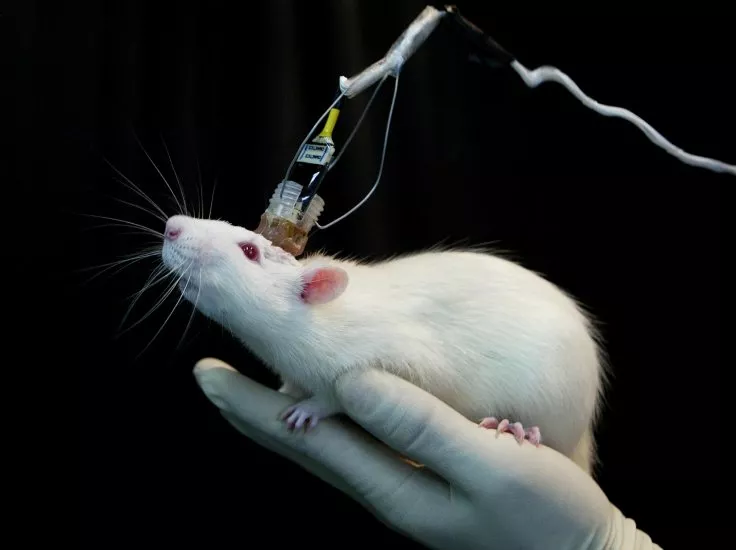
\includegraphics[width=\textwidth]{figures/scientist-deep-brain-stimulation.png}
    \caption[Depiction of a rat with an electrode implant]{Depiction of a rat with an electrode implant \citep{sharma_scientists_2017}.}
    \label{fig:dbs-implant}
  \end{figure}

  Animal models, in this case, rats, provide a more realistic portrayal of the effects of an intervention as they allow for the study of the intervention’s impact on a living organism, replicating a more natural environment and providing a closer approximation to human physiology than in vitro methods.

  Twenty male albino Sprague Dawley rats underwent electrode implantation (exemplary depiction in \autoref{fig:dbs-implant}) and stimulation sessions. After the stimulation, the rats’ brains were removed and processed to determine the location of the electrode tips.

  The use of animal models in this research created a safe and controlled environment to study the effects of subthalamic stimulation on the brain, yielding valuable insights and emphasising the critical role that animal models play in neuroscience research.

  \subsection{Gene Silencing in Huntington’s Disease}
  \label{sec:huntingtons}

  Huntington’s disease affects movement, thinking, and behaviour and can impact the structure of the human brain, as shown in \autoref{fig:huntingtons}. In a study by \cite{savas_huntingtons_2008}, mice brains were used to study the role of Ago proteins in RNA-mediated gene silencing pathways. Brain cells from normal mice and mice with a specific genetic mutation were studied to understand the differences in Ago proteins.

  \begin{figure}[ht]
    \centering
    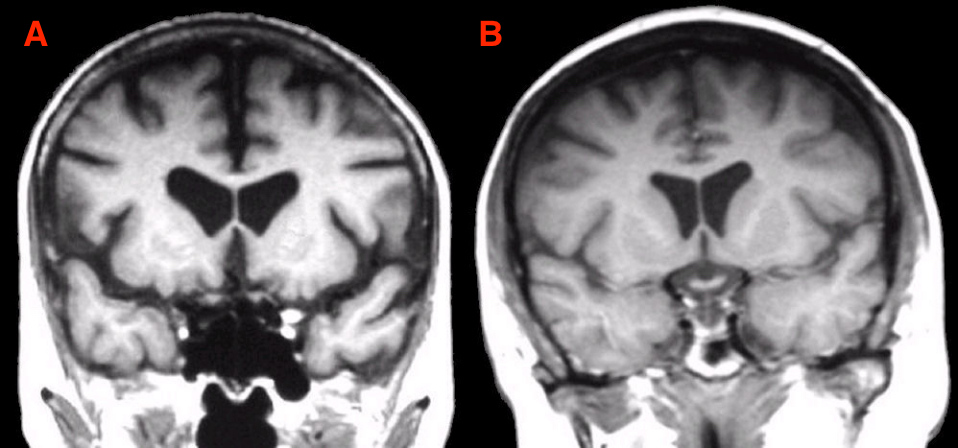
\includegraphics[width=\textwidth]{figures/huntington.jpg}
    \caption[Brain scan of the caudate nucleus in two different conditions, (A) represents a patient diagnosed with Huntington’s disease, while (B) represents a patient without the condition]{Brain scan of the caudate nucleus in two different conditions, (A) represents a patient diagnosed with Huntington’s disease, while (B) represents a patient without the condition \citep{c_preston_huntingtons_nodate}.}
    \label{fig:huntingtons}
  \end{figure}

  The findings from this study may have implications for understanding the pathogenesis of Huntington’s disease in humans. The analysis studied the impact of a specific genetic mutation, known as mutant Htt, on a protein called Ago2. The results suggest that the presence of mutant Htt reduces the amount of Ago2 that enters structures within cells called P bodies. This reduction in the amount of Ago2 entering P bodies could result in changes to the number and behaviour of these structures over time and may help to explain the long period it takes for the disease to manifest in patients. This research shows the importance of animal models in helping us better understand diseases like Huntington’s. Animal models give us access to large amounts of information that can be used to identify other essential proteins and molecules and to study how genetics and the environment affect the development and behaviour of organisms.

  \section{Shortcomings of Animal Models}
  \label{sec:shortcomings}

  \vspace{10pt} % Increase vertical spacing before figure
  \begin{figure}[ht]
    \centering
    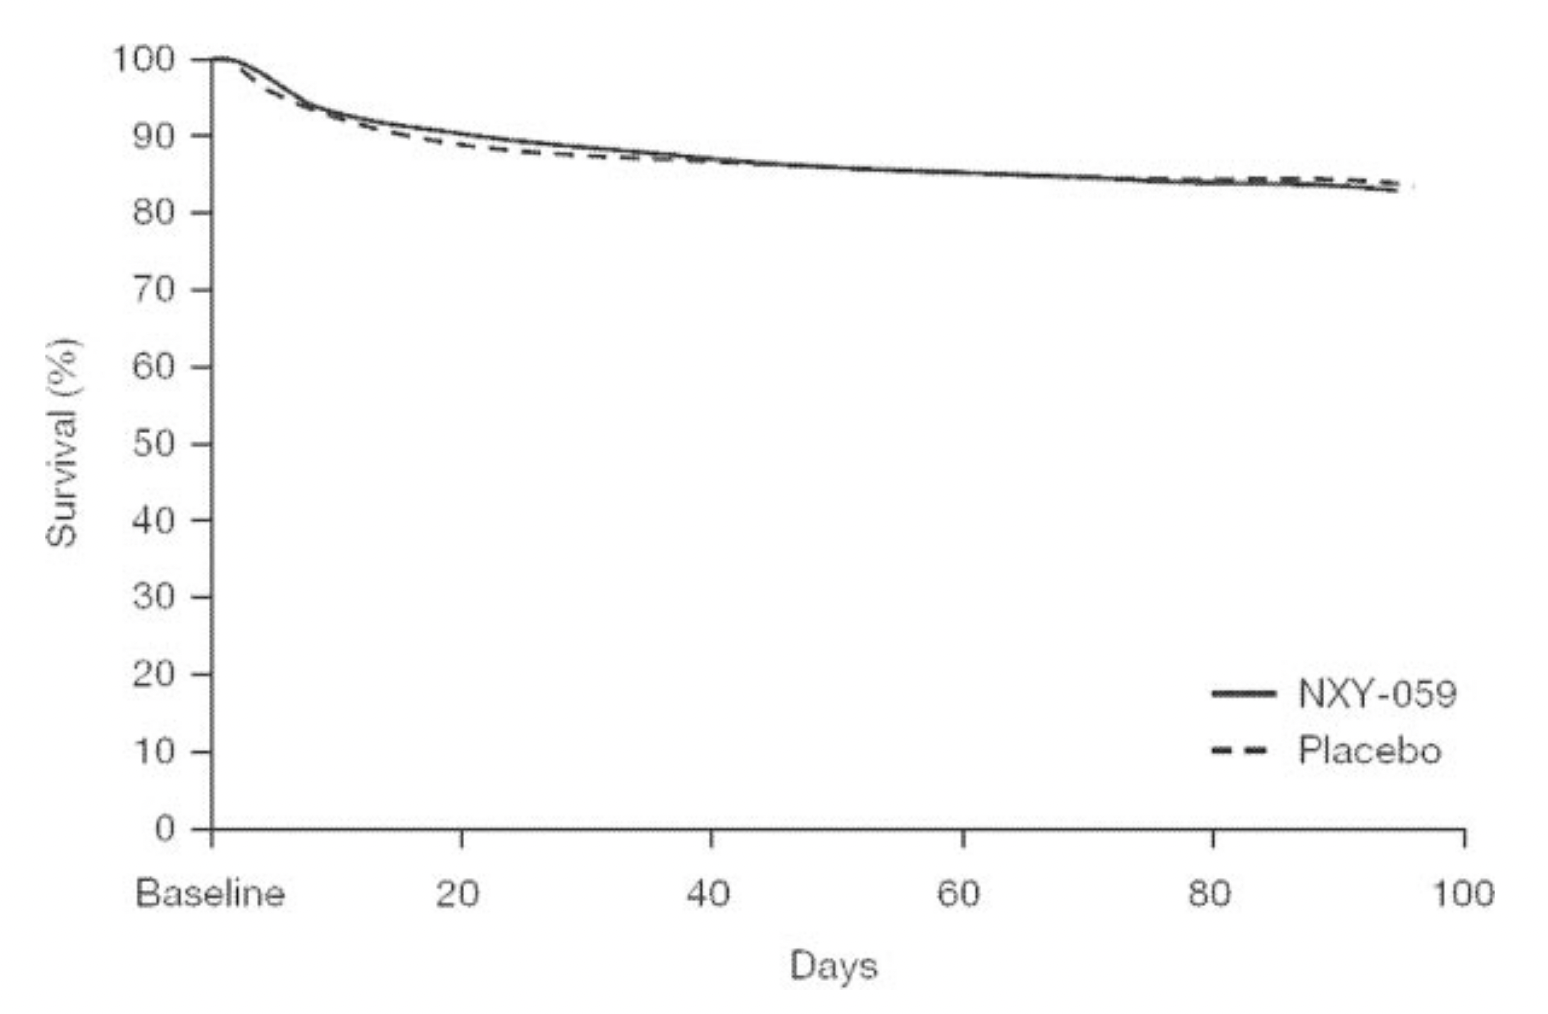
\includegraphics[width=\textwidth]{figures/death-rates.png}
    \caption[Comparison of death rates: The results reveal a similar number of deaths among patients treated with NXY-059 (16.6\%) and those receiving a placebo (16.4\%), indicating limited effectiveness of the medication]{Comparison of death rates: The results reveal a similar number of deaths among patients treated with NXY-059 (16.6\%) and those receiving a placebo (16.4\%), indicating limited effectiveness of the medication \citep{diener_nxy-059_2008}.}
    \label{fig:death-rates}
  \end{figure}

  In the previous chapter, we discussed two examples of animal models that have been incredibly valuable in furthering our understanding of diseases and developing new treatments. However, while animal models can provide valuable insights, they can sometimes fail to accurately predict treatments’ effects in human patients.

  One example is the research paper “NXY-059 for the Treatment of Acute Stroke” by \cite{diener_nxy-059_2008}. This paper investigated the efficacy of NXY-059, a medication, in patients with Acute Ischemic Stroke (AIS). The study enrolled patients with stroke from May 2003 through June 2006 and included a randomised, double-blind, placebo-controlled study and a pooled analysis of the two studies as depicted in \autoref{fig:death-rates}.

  The results of the clinical trials in stroke patients did not match the results of preclinical animal studies, which explored the role of NXY-059 in rats and small primates. The study suggests that the differences could be due to the different ways the studies were conducted and limitations in medical imaging technology at the time. This shows that it is important to use animal models as part of a larger research plan but not to rely solely on them. In order to accurately predict the effects of treatments, it is important to conduct rigorous clinical trials and use various research methods.

  \section{Combination of Different Research Methods}
  \label{sec:discussion}

  Despite the efficacy of animal models in controlled environments, it must be acknowledged that these models have limitations. The fundamental differences between species, even those as closely related as primates and humans, can fail to accurately predict treatments’ effects in human patients. Moreover, the ethical concerns surrounding the use of animals in research must be addressed, as significant numbers of animals are used and discarded every year without yielding meaningful results. Furthermore, exploring the reasons why certain animal models are preferred over others, such as mice, rats, drosophila, zebrafish, and macaques, would be a thought-provoking topic for further discussion or a separate essay \citep{govuk_statistics_2022}.

  \vspace{10pt} % Increase vertical spacing before figure
  \begin{figure}[ht]
    \centering
    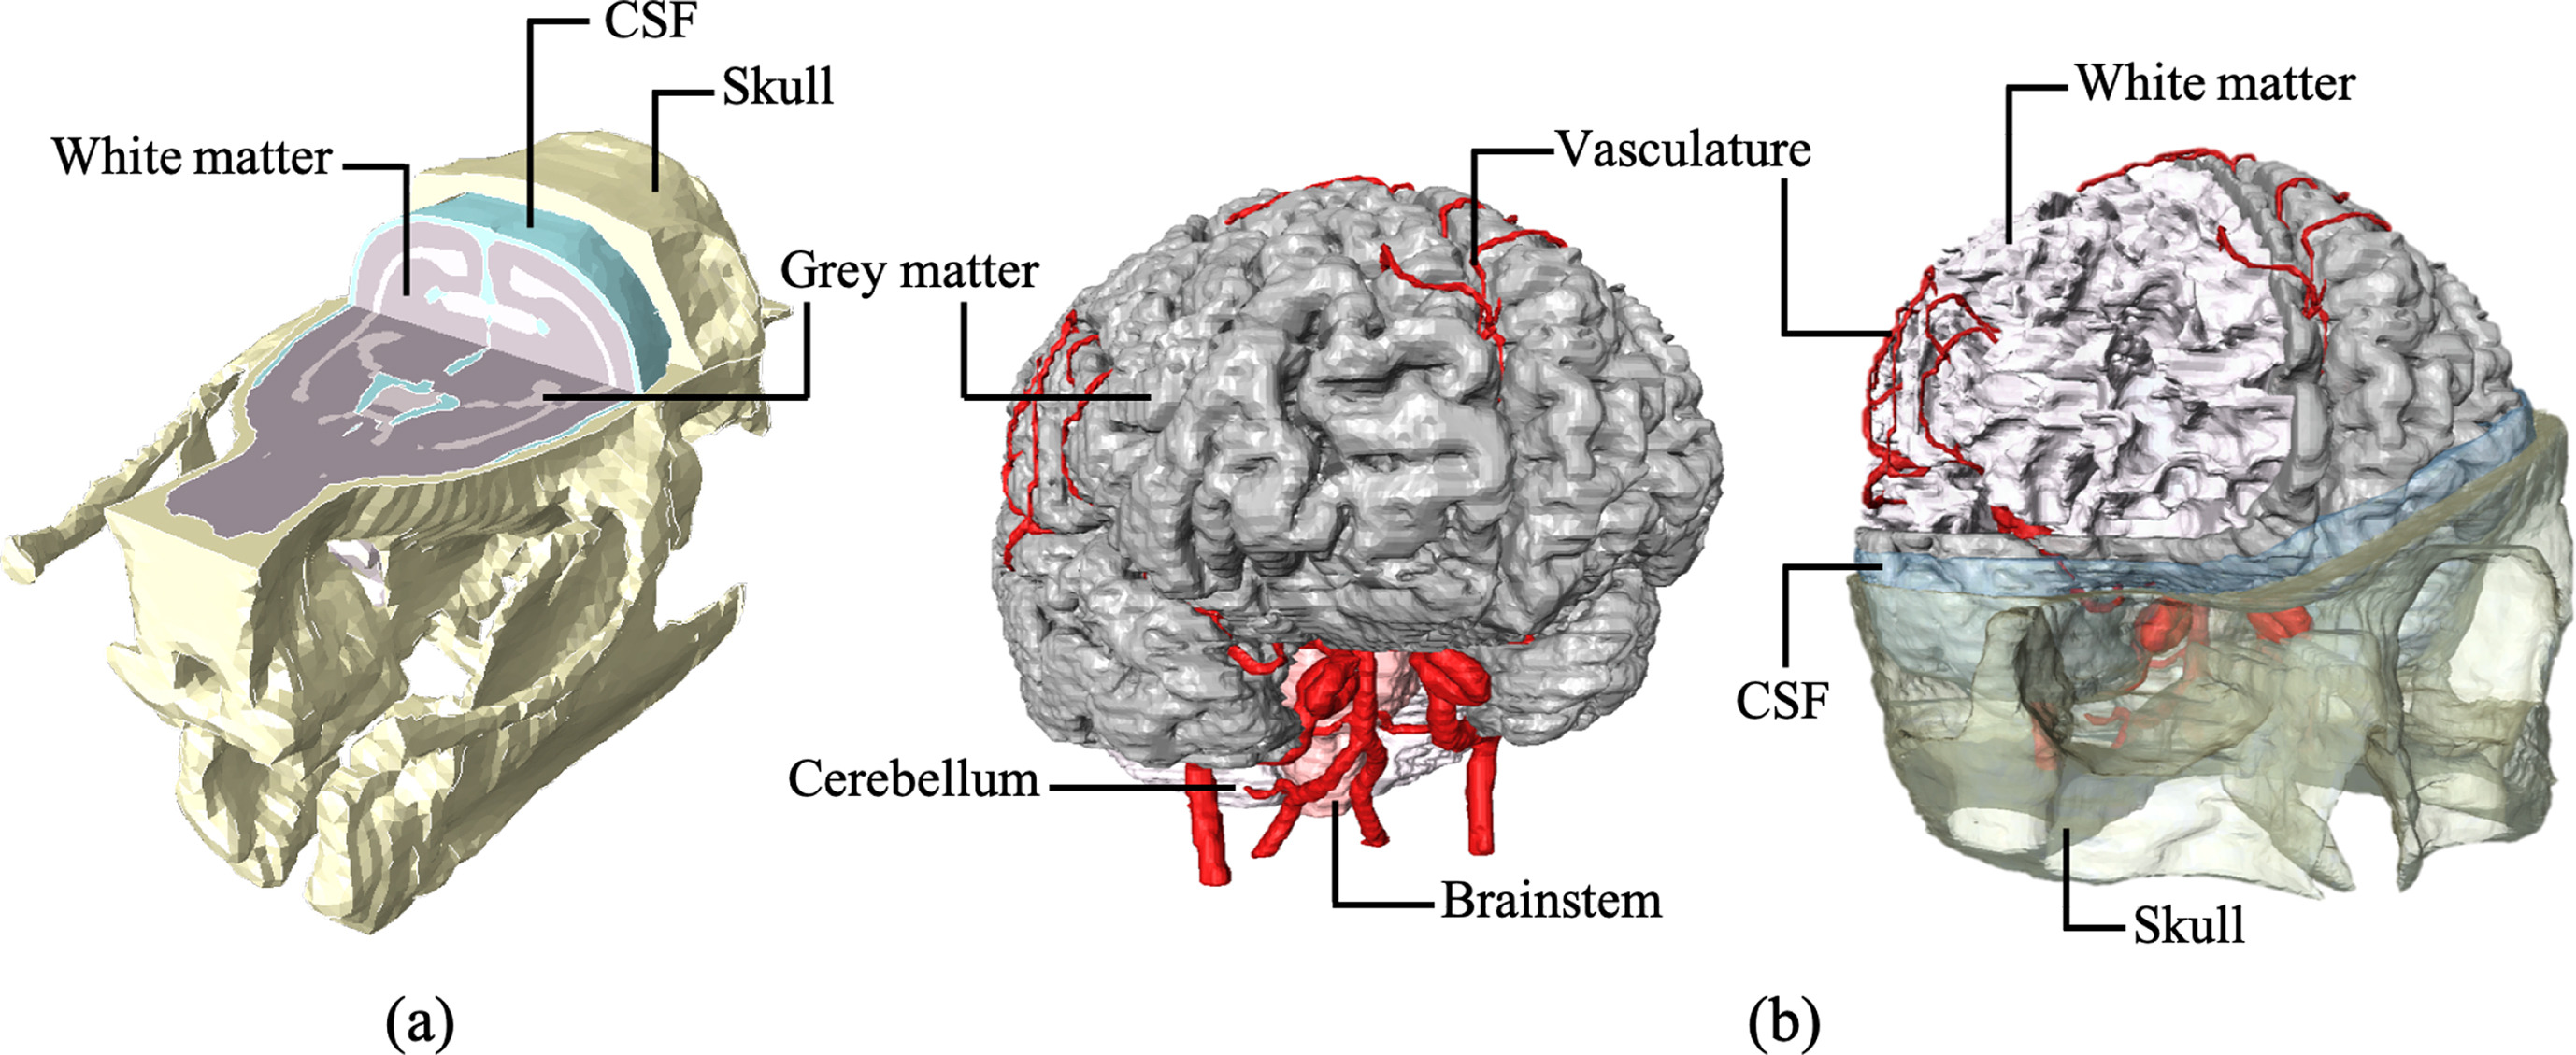
\includegraphics[width=\textwidth]{figures/in-silico.jpg}
    \caption[Simulation of a stroke using numerical models of a rat head and a human head]{Simulation of a stroke using numerical models of a rat head (b) and a human head (b) \citep{bing_medical_2020}.}
    \label{fig:silico}
  \end{figure}

  In response to these limitations, the utilisation of alternative models is increasingly being recommended by the scientific community. In vitro cell cultures, for instance, offer a means of studying biological processes in neurons without the use of live animals, while in silico models, which simulate neuronal structures on computers, have demonstrated success in recent research, such as in the research on strokes \citep{bing_medical_2020} as depicted in \autoref{fig:silico}. Another promising avenue is using brain organoids, such as the neurospheres developed by Swiss startup FinalSpark as depicted in \autoref{fig:neurospheres}, which can provide valuable insights into bidirectional neural interfacing without the need for living in vivo animal models \citep{finalspark_artificial_2022}.

  \vspace{10pt} % Increase vertical spacing before figure
  \begin{figure}[ht]
    \centering
    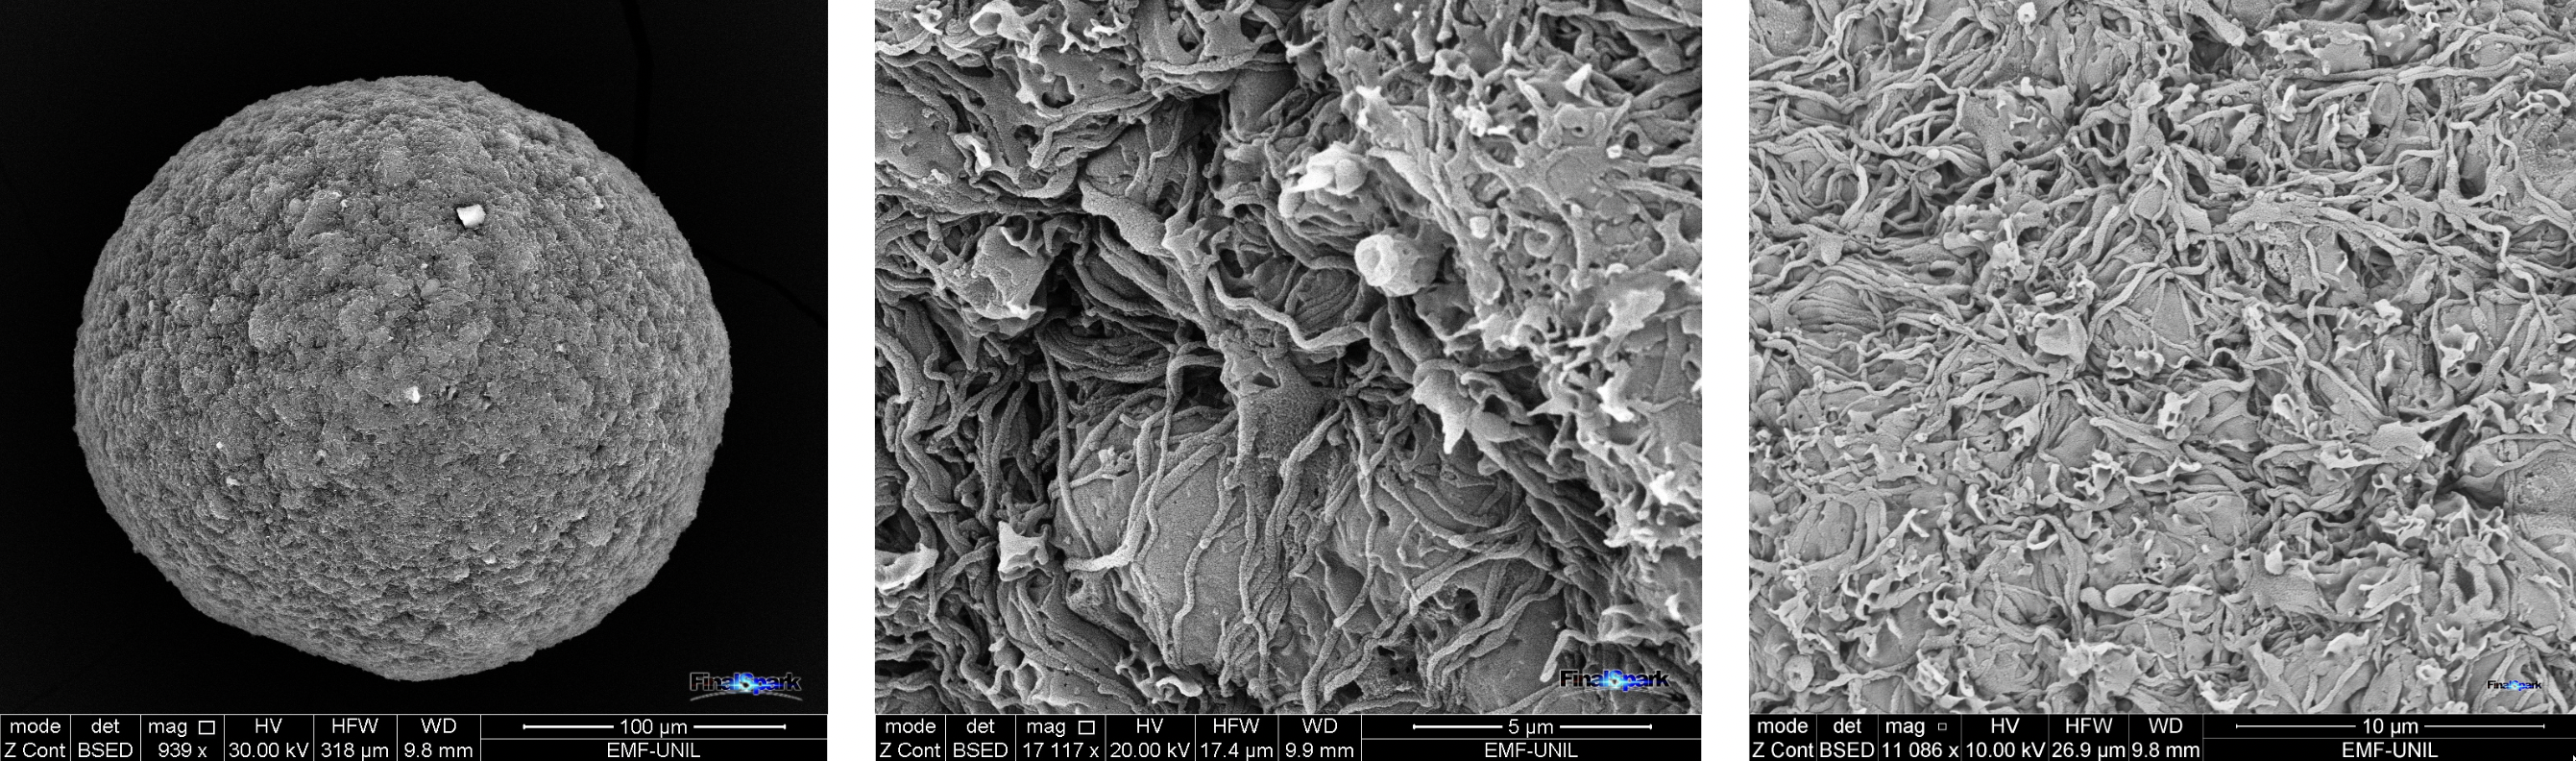
\includegraphics[width=\textwidth]{figures/neurosphere.png}
    \caption[Photographs of a neurosphere developed by the Swiss company FinalSpark]{Photograph of a neurosphere developed by the Swiss company FinalSpark \citep{finalspark_artificial_2022}.}
    \label{fig:neurospheres}
  \end{figure}

  It becomes clear that by incorporating alternative models, including in vitro cell cultures, in silico models, and brain organoids, into our research paradigms, we can understand the effects of treatments, thus mitigating the reliance on animal models and advancing the field of medical research.

  \section{Conclusion}
  \label{sec:conclusion}

  This essay examined two cases in which animal models were beneficial for studying diseases related to the human brain and one example in which they were not.

  In recent years, alternative models such as in vitro cell cultures, in silico models, and brain organoids (e.g. neurospheres, sometimes also referred to as organ-on-a-chip \citep{huh_reconstituting_2010}) have gained increased attention in medical research. Such engineered models offer advantages such as the ability to study biological processes without using animals, simulate neural structures on computers by precisely altering the needed features, and provide valuable insights into certain aspects of cells and organisms.

  \begin{figure}[ht]
    \centering
    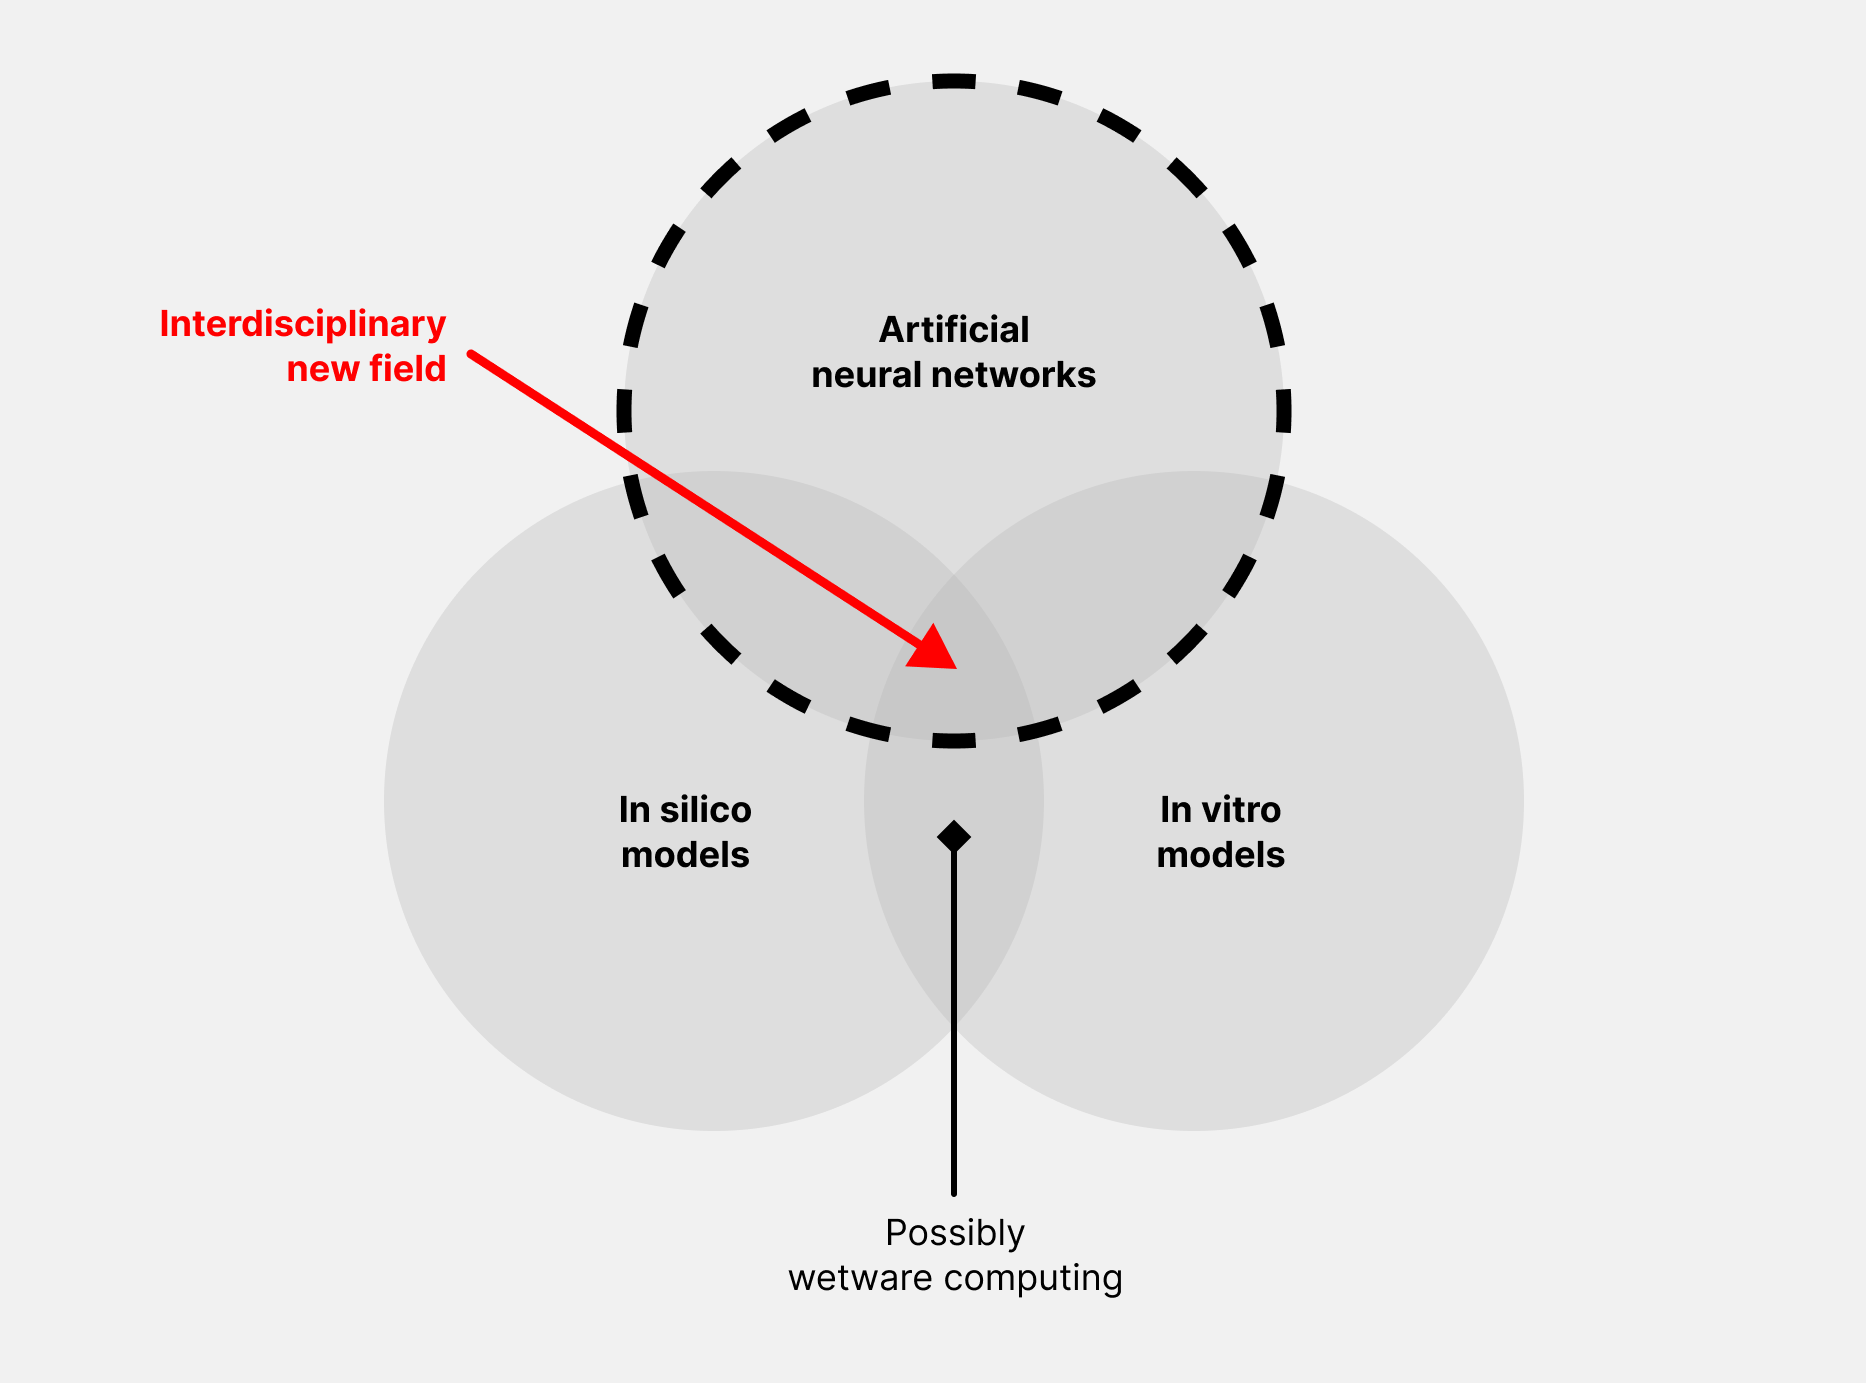
\includegraphics[width=\textwidth]{figures/new-discipline.png}
    \caption[Illustration showing the intersection of a possibly new interdisciplinary research field combining artificial neural networks and in vitro as well as in silico models.]{Illustration showing the intersection of a possibly new interdisciplinary research field combining artificial neural networks and in vitro as well as in silico models.}
    \label{fig:new-discipline}
  \end{figure}

  The author suggests that an interdisciplinary approach, as depicted in \autoref{fig:new-discipline}, combining these models could lead to even more comprehensive and accurate results. For instance, stimulating brain organoids via neural interfaces and combining this with in silico models could provide a complete understanding of the effects of treatments in a virtual environment. With the increased push in the fields of artificial neural networks and wetware computing, such an interdisciplinary field may arise in the near future, leading to a more thorough and ethical understanding of the human brain and neurological diseases.

  \pagebreak
  \singlespacing % No need for double spacing in the references
  \bibliographystyle{references/custom-apa}
  \bibliography{references/bibliography}

\end{sloppypar}
\end{document}